This module visualizes the calculated points and the camera positions relative to the position of the first camera. This part of the program is written on top of the OpenGL graphics API.

It can be run as a stand alone program, or as a last step in the 3D-reconstruction pipline. In the standalone case it will read the output files generated by the reconstruction pipeline. Using the keyboard a user can then step between the added cameras, with or without the bundle adjustment step done.

It is also possible to alter the scale of the points and cameras, as there is no automatic scaling in place and the points are drawn as colored spheres.

%massa bilder här, nån får ta och "fota" dem.

\subsubsection{Visualization}
The estimated 3D-points are plotted as textured/colored spheres, using the color from the image where the corresponding interest point was first detected, or a region surrounding the point. (this looks rather bad however)

Cameras are plotted as cones pointing toward the point cloud.

\begin{figure}[htb]
	\centering
	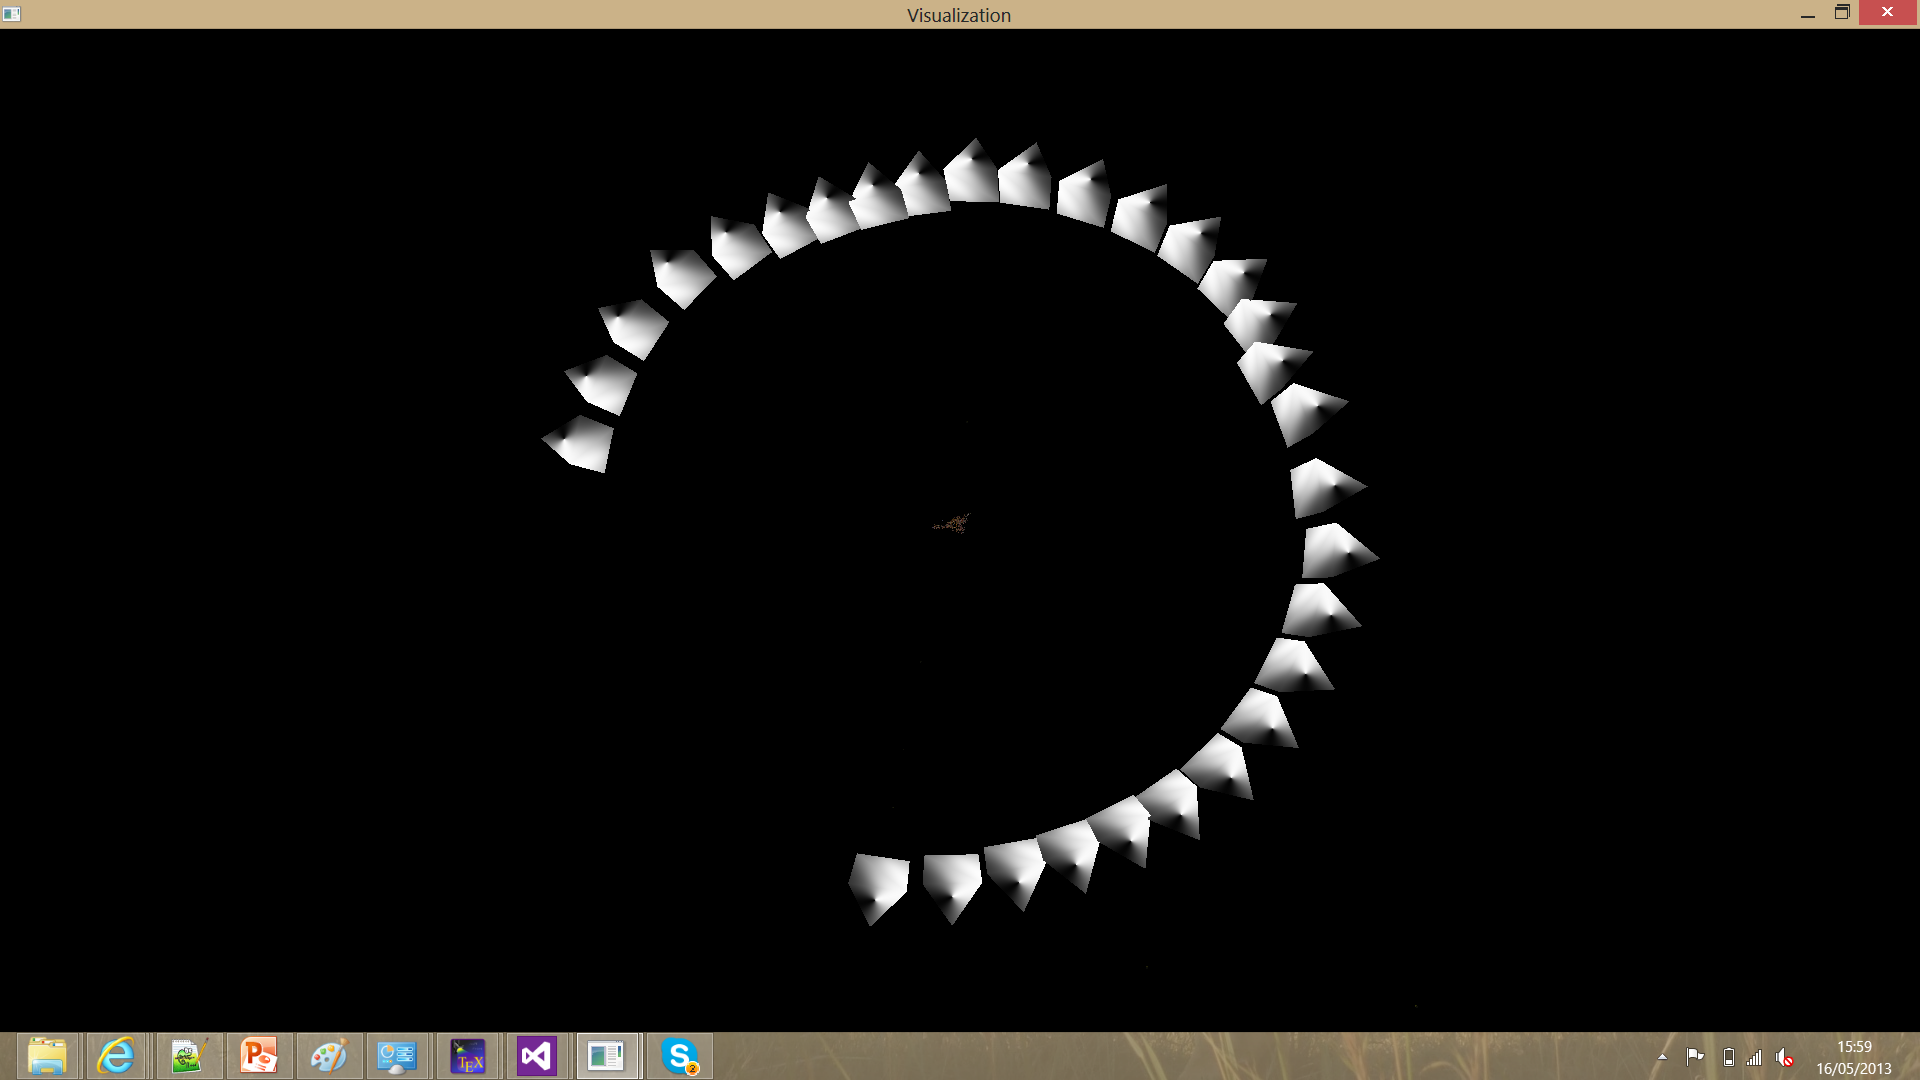
\includegraphics[width=110mm]{images/camRingLots.png}
	\caption{\textit{some cameras}}
	\label{fig:camRingLots}  %Skapar referens till figuren
\end{figure}

\begin{figure}[htb]
	\centering
	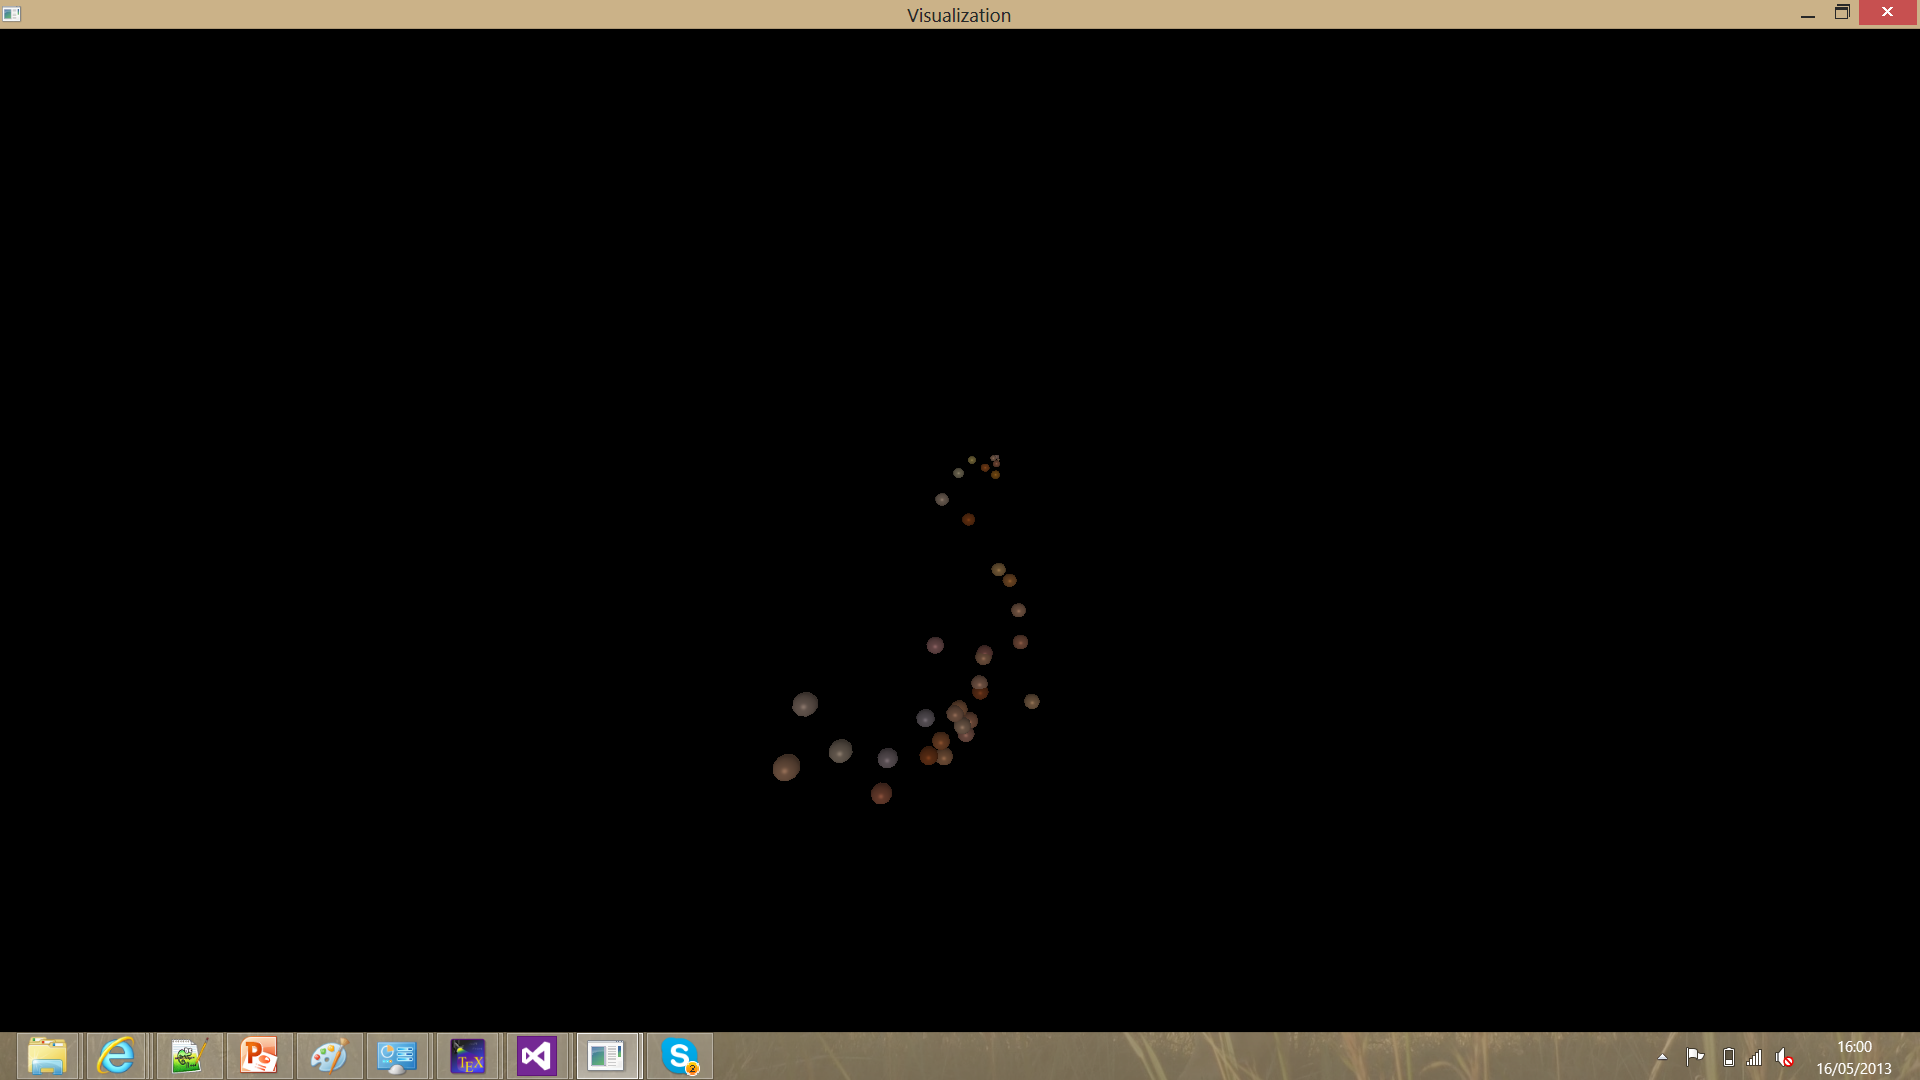
\includegraphics[width=110mm]{images/pointCloudFewCam.png}
	\caption{\textit{The dinosoaur with only a few cameras, very poor depth accuracy}}
	\label{fig:camRingLots}  %Skapar referens till figuren
\end{figure}

The main purpouse of the visualization modue is to compare 


\subsubsection{File managing}
Each iteration of the reconstruction pipeline produces two files, one with the reconstruction state before the bunle adjustment and one after. The files contain all detected 2D correspondances, the calculated fundamental matrix, and the known 3D points. The data is saved as text, to make inspection easier.
